% !TeX spellcheck = ru_RU_yo
% !TEX program = xelatex

\documentclass[pta]{../../../scs-iam}

\begin{document}

\newgeometry{
  top=20mm,
  right=15mm,
  bottom=20mm,
  left=20mm,
  bindingoffset=0cm
}

\thispagestyle{empty}

\begin{center}
  {
    \bfseries
    {
      \subnormal
      Министерство образования и науки Российской Федерации
    } \\[-0.5em]
    {
      \scriptsize
      ФЕДЕРАЛЬНОЕ ГОСУДАРСТВЕННОЕ АВТОНОМНОЕ ОБРАЗОВАТЕЛЬНОЕ УЧРЕЖДЕНИЕ ВЫСШЕГО ОБРАЗОВАНИЯ
    } \\[-0.25em]
    {
      \subnormal
      “САНКТ-ПЕТЕРБУРГСКИЙ НАЦИОНАЛЬНЫЙ ИССЛЕДОВАТЕЛЬСКИЙ \\[-0.5em]
      УНИВЕРСИТЕТ ИНФОРМАЦИОННЫХ ТЕХНОЛОГИЙ, \\[-0.75em]
      МЕХАНИКИ И ОПТИКИ”
    } \\[1em]
  }
  \begin{minipage}{.8\textwidth}
    \titledline{\textbf{Факультет}}
    $\underset{
      \text{\scriptsize (название факультета)}
    }{
      \underline{\makebox[\remaining][c]{программной инженерии и компьютерной техники}}
    }$ \\
    \textbf{Кафедра}
    \hfill
    $\underset{
      \text{\scriptsize (название кафедры)}
    }{
      \underline{\makebox[\remaining][c]{информатики и прикладной математики}}
    }$ \\[-0.5em]
    \titledline{\textbf{Направление подготовки (специальность)}}
    \underline{\makebox[\remaining][c]{\strut 09.04.01~~}}
  \end{minipage}
\end{center}

\small

\begin{center}
  {
    \normalsize
    \textbf{О Т Ч Ё Т}
  } \\[-0.25em]
  \textbf{о}~$\underset{\text{\scriptsize (название практики)}}{\underline{\makebox[.42\textwidth][c]{производственной (преддипломной)}}}$~\textbf{практике}
\end{center}

{
  \parindent 0pt
  
  \textbf{Тема задания}
  \uline{<<Разработка архитектуры клиентской части веб-приложения для работы с устрой\-ствами Emlid Reach и Emlid Reach RS>> \hfill} \\[-1em]
  
  \textbf{Студент}
  $\underset{
    \text{\scriptsize (Фамилия, Имя, Отчество)}
  }{
    \underline{\makebox[.65\textwidth][l]{Кузнецов Андрей Андреевич}}
  }$
  \hfill
  \textbf{Группа №}
  \underline{\makebox[.1\textwidth][c]{\strut P4215~~}} \\[-1em]
  
  \titledline{\textbf{Руководитель практики от организации}}
  $\underset{
    \text{\scriptsize (Фамилия И.О., должность и место работы)}
  }{
    \underline{\makebox[\remaining][s]{Фёдоров Е.М., ИП Николаев Д.А., руководитель от-}}
  }$
  \uline{дела разработки программного обеспечения\hfill} \\[-1em]
  
  \titledline{\textbf{Руководитель практики от университета}}
  $\underset{
    \text{\scriptsize (Фамилия И.О., должность)}
  }{
    \underline{\makebox[\remaining][l]{Исаев И.В., ассистент}}
  }$ \\[1.5em]
  
  \begin{flushright}
    \begin{minipage}{.5\textwidth}
      \titledline{\textbf{Практика пройдена с оценкой}}
      \underline{\makebox[\remaining][c]{}} \\[-1em]

      \textbf{Подписи членов комиссии}\\
      \signature\hfill
      $\underset{
        \text{\scriptsize (Фамилия И.О.)}
      }{
        \underline{\makebox[12em][s]{\strut}}
      }$ \\
      \signature\hfill
      $\underset{
        \text{\scriptsize (Фамилия И.О.)}
      }{
        \underline{\makebox[12em][s]{\strut}}
      }$ \\
      \signature\hfill
      $\underset{
        \text{\scriptsize (Фамилия И.О.)}
      }{
        \underline{\makebox[12em][s]{\strut}}
      }$ \\[0.5em]
    
      \textbf{Дата}~\datetemplate
    \end{minipage}
  \end{flushright}
}

\vfill

\begin{center}
  {
    \normalsize
    Санкт-Петербург \\
    2018 г.
  }
\end{center}

\restoregeometry
\normalsize

\clearpage

\setcounter{page}{2}

\section*{СОДЕРЖАНИЕ}
\tableofcontents

\newpage

\mysection{ОБЩИЕ СВЕДЕНИЯ}

С 30 апреля по 3 июня 2018 года обучающийся проходил производственную практику в ИП Николаев Денис Александрович. На практику было дано задание по разработке архитектуры веб-приложения для управления ГНСС-приёмниками, работающими под управлением программного обеспечения, основанного на программном комплексе высокоточного позиционирования RTKLIB.

В процессе прохождения практики были изучены следующие электронные источники и литература:
\begin{dashitemize}
  \item документация программного комплекса RTKLIB;
  \item документация устройств Emlid Reach и Emlid Reach RS;
  \item техническое задание на разработку программного модуля.
\end{dashitemize}

\mysection{ХОД РАБОТЫ}

\subsection{Этап 1 -- Платформа для разработки}

Платформой для разработки являлись устройства Emlid Reach и Emlid Reach RS. Данные ГНСС-приёмники работают под управлением программного обеспечения, основанного на программном комплексе высокоточного позиционирования RTKLIB. Работа пользователя с данными продуктами осуществляется через веб-приложение, доступ к которому можно получить с помощью любого устройства, на котором установлен веб-браузер.

Reach и~Reach~RS созданы на базе одного и~того же вычислительного модуля и~используют одинаковые приёмники u-blox, имеется ряд существенных различий в~аппаратном обеспечении данных устройств. Различия Reach и~Reach~RS, которые необходимо учесть при создании архитектуры веб-приложения, указаны в~таблице \ref{tab:reach-vs-reachrs}.

\ctable[
pos=h!,
caption={Различия Reach и~Reach~RS},
label={tab:reach-vs-reachrs}
]{|l|*{2}{>{\centering\arraybackslash}m{2.3cm}|}}{}{
  \toprule
  \multicolumn{1}{|c|}{\textbf{Техническая особенность}} & \textbf{Reach} & \textbf{Reach~RS} \\
  \midrule
  Встроенная батарея & нет & да \\
  \midrule
  Встроенная антенна & нет & да \\
  \midrule
  Встроенное радио & нет & да \\
  \midrule
  Физическая кнопка на корпусе & нет & да \\
  \midrule
  Возможность управления фотокамерой & да & нет \\
  \bottomrule
}

\subsection{Этап 2 -- Постановка задачи работы}

Основной задачей производственной практики являлось создание архитектуры веб-приложения, необходимого для осуществления взаимодействия пользователя с вышеупомянутыми ГНСС-приёмниками.

\subsection{Этап 3 -- Проектирование приложения}

\subsubsection{Основные задачи и требования}

Для создания общей архитектуры приложения были сформулированы наиболее важные идеи, задачи и~требования, предъявляемые к~разрабатываемому продукту.

Важно отметить, что в~следующем далее списке присутствуют пункты, которые касаются лишь разработчиков программных компонентов, отвечающих за взаимодействие с~RTKLIB, системными утилитами и~различными аппаратными компонентами Reach и~Reach~RS. Данные модули и~детали их разработки выходят за рамки рассматриваемой работы, но являются важными для понимания общей структуры приложения.

Разрабатываемое приложение должно:

\begin{dashitemize}
  \item \textbf{Осуществлять запуск приложений RTKLIB в~управляемых контейнерах}. Надёжным и~простым способом организации взаимодействия с~приложениями RTKLIB является их запуск в~управляемых контейнерах. При данном подходе необходимые утилиты будут работать так же, как если бы пользователь запускал их в~терминале.

  Используя подобный подход, становится возможно организовать взаимодействие веб-приложения с~необходимыми программами таким образом, что:

  \begin{dashitemize}
    \item не требуется вмешательство в~исходный код RTKLIB;
    \item облегчается поддержка совместимости с~новыми версиями программного комплекса;
    \item разрабатываемый продукт остаётся независим от изменений в~кодовой базе RTKLIB. 
  \end{dashitemize}

  \item \textbf{Иметь клиентскую часть, представленную в~виде одностраничного приложения}. Как показал проведённый обзор, данный подход в~настоящее время является одним из самых популярных решений для создания веб-интерфейсов, предназначенных для управления такими устройствами, как Reach или Reach~RS.

  \item \textbf{Поддерживать передачу данных по протоколу WebSocket}. Для создания отзывчивого интерфейса веб-приложения и~обеспечения лучшего пользовательского опыта б\`{о}льшую часть взаимодействий клиентской части с~сервером следует организовать с~помощью асинхронных запросов и~сообщений.

  Наиболее удачным решение для разрабатываемого приложения является протокол WebSocket. Создавая на клиентской части веб-приложения слушателей определённых событий, становится возможно организовать отображение различной информации в~режиме реального времени без постоянных опросов сервера.
\end{dashitemize}

\subsubsection{Основные модули}

Перечислим основные модули приложения (рис.~\ref{fig:raw-system-architecture}):

\begin{alphitemize}
  \item Серверная часть
  \begin{alphitemize}
    \item WebSocket сервер
    \item Модуль взаимодействия с~RTKLIB
    \item Демоны и~сервисы для взаимодействия с~аппаратными компонентами устройства
  \end{alphitemize}
  
  \item Клиентская часть
  \begin{alphitemize}
    \item WebSocket клиент
    \item JavaScript-приложение
  \end{alphitemize}
\end{alphitemize}

\begin{figure}[h!]
  \centering
  \setlength{\fboxsep}{5pt}
  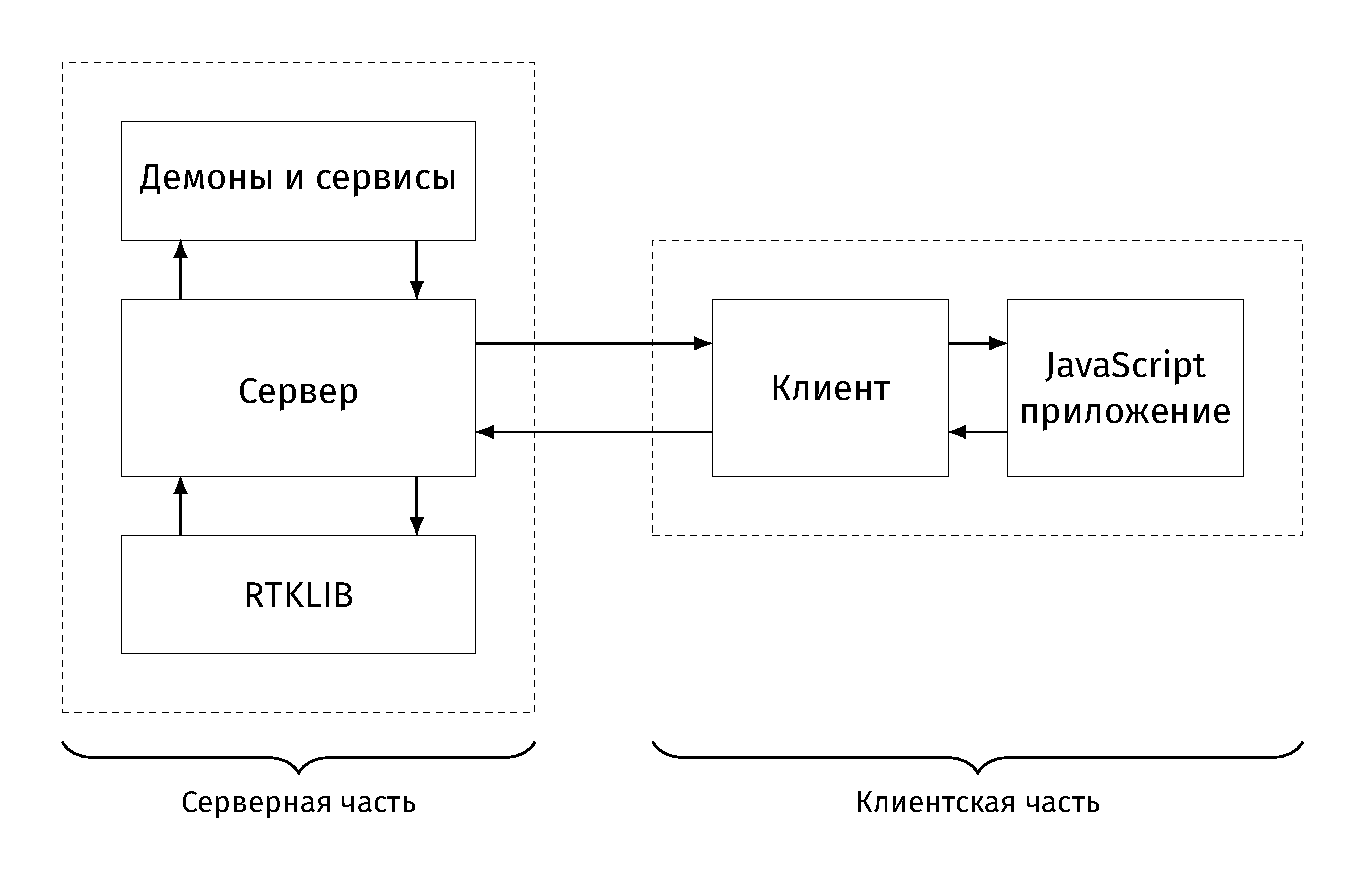
\includegraphics[width=\textwidth]{../../../img/tikz/raw-system-architecture/pic}
  \vspace*{12pt}
  \caption{Общая архитектура приложения}\label{fig:raw-system-architecture}
\end{figure}

\subsubsection{Выбор инструментов разработки}

\paragraph{Серверная часть приложения}

В~рамках разработки описанного приложения выбор инструментов для написания серверной части приложения зависит не только от возможностей веб-фреймворков, доступных для того или иного языка программирования, но и~от задач, описанных в~пункте 2.3.1. Также, важно помнить, что разрабатываемое приложение предназначено для запуска на устройствах с~ограниченными вычислительными ресурсами.

Разработчиками серверной части приложения был проведён обзор высокоуровневых языков программирования, часто используемых для разработки веб-приложений. Основными из рассмотренных вариантов были языки Java, Python и~Ruby.

На основании различных оценок, детали формирования которых выходят за рамки рассматриваемой работы, основным языком для серверной части приложения был выбран Python.

Одним из основных инструментов при написании серверной части приложения был выбран веб-фреймворк Flask. Запуск приложений RTKLIB в~управляемых контейнерах осуществляется с~помощью модуля pexpect.

\paragraph{Клиентская часть приложения}

Основу клиентской части приложения составляют: язык гипертекстовой разметки HTML, CSS-стили и~скрипты на языке JavaScript.

Для наиболее быстрой и~удобной разработки одностраничного приложения было решено использовать специализированную библиотеку или фреймворк. На момент проектирования приложения одними из самых популярных инструментов для создания одностраничных приложений являлись React, Angular 2 и~Vue.js.

Для анализа и сравнения вышеперечисленных библиотек и фреймворков были изучены:
\begin{dashitemize}
  \item официальные документации;
  \item исходные коды простейших приложений и~их компонентов;
  \item результаты синтетических тестов.
\end{dashitemize}

По результатам изучения возможных решений для разработки приложения был выбран фреймворк Vue.js. Данный выбор также был обусловлен наличием у автора данной работы опыта разработки с~использованием фреймворка AngularJS, который является одним из источников вдохновения для создателей Vue.js.

Также, вместе с~Vue.js было решено использовать библиотеку-расши-рение для данного фреймворка -- Vuex. Данная библиотека позволяет создать централизованное хранилище данных, доступ к~которому будут иметь все компоненты приложения. Одной из важнейших особенностей работы с~таким хранилищем является способность компонентов Vue.js реактивно обновлять своё состояние при изменении тех или иных данных в~Vuex.

\subsection{Детализированная архитектура приложения}
\label{subsec:app-architecture}

С~учётом инструментов, выбранных в~предыдущем подразделе, уточним архитектуру приложения, представленную ранее (рис.~\ref{fig:raw-system-architecture}). На рисунке \ref{fig:complete-system-architecture} изображена детализированная архитектура разрабатываемого приложения.

\begin{figure}[h!]
  \centering
  \setlength{\fboxsep}{5pt}
  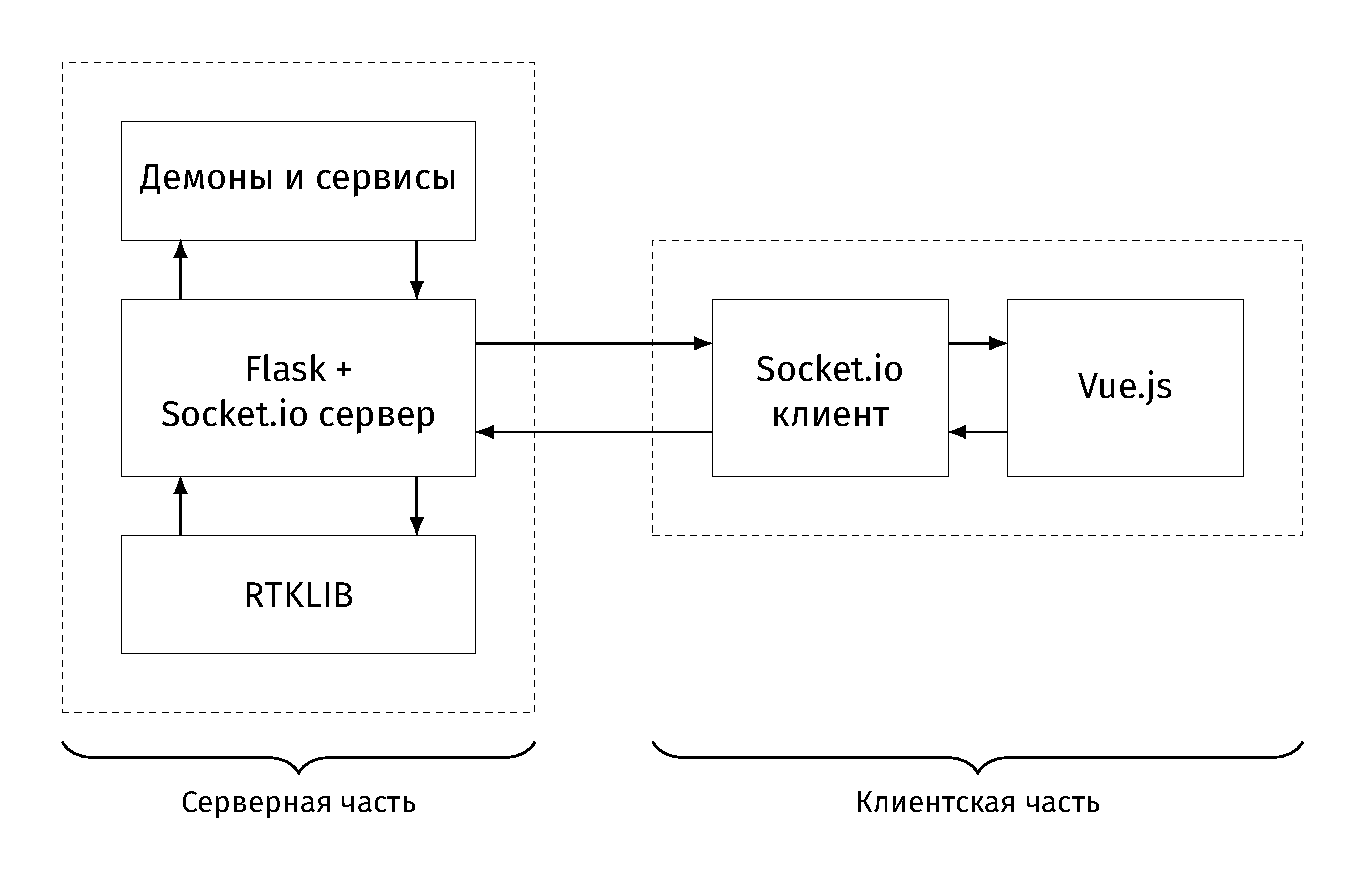
\includegraphics[width=\textwidth]{../../../img/tikz/system-architecture/pic_sans_no-border}
  % \vspace*{12pt}
  \caption{Детализированная архитектура приложения}\label{fig:complete-system-architecture}
\end{figure}

\subsubsection{Подробная архитектура клиентской части приложения}

Клиентская часть разрабатываемого приложения представляет из себя совокупность отдельных программных модулей и глобального хранилища, изменения данных в котором вызывают реактивное обновление модулей, имеющих соответствующие слушатели событий.

Модули приложения можно условно разделить на две группы:
\begin{dashitemize}
  \item модули, являющиеся \emph{моделями представления} для соответствующих экранов приложения;
  \item модули общего назначения, предназначенные для обработки событий, приходящих от сервера, или содержащие различные утилиты.
\end{dashitemize}

На рисунке \ref{fig:fe-architecture} изображены все основные компоненты приложения и их связи с глобальным хранилищем. К модулям общего назначения относятся только модуль обработки событий и модуль работы с картами, остальные компоненты написаны с помощью Vue.js и связаны с представлениями приложения.

\begin{figure}[h!]
  \centering
  \setlength{\fboxsep}{5pt}
  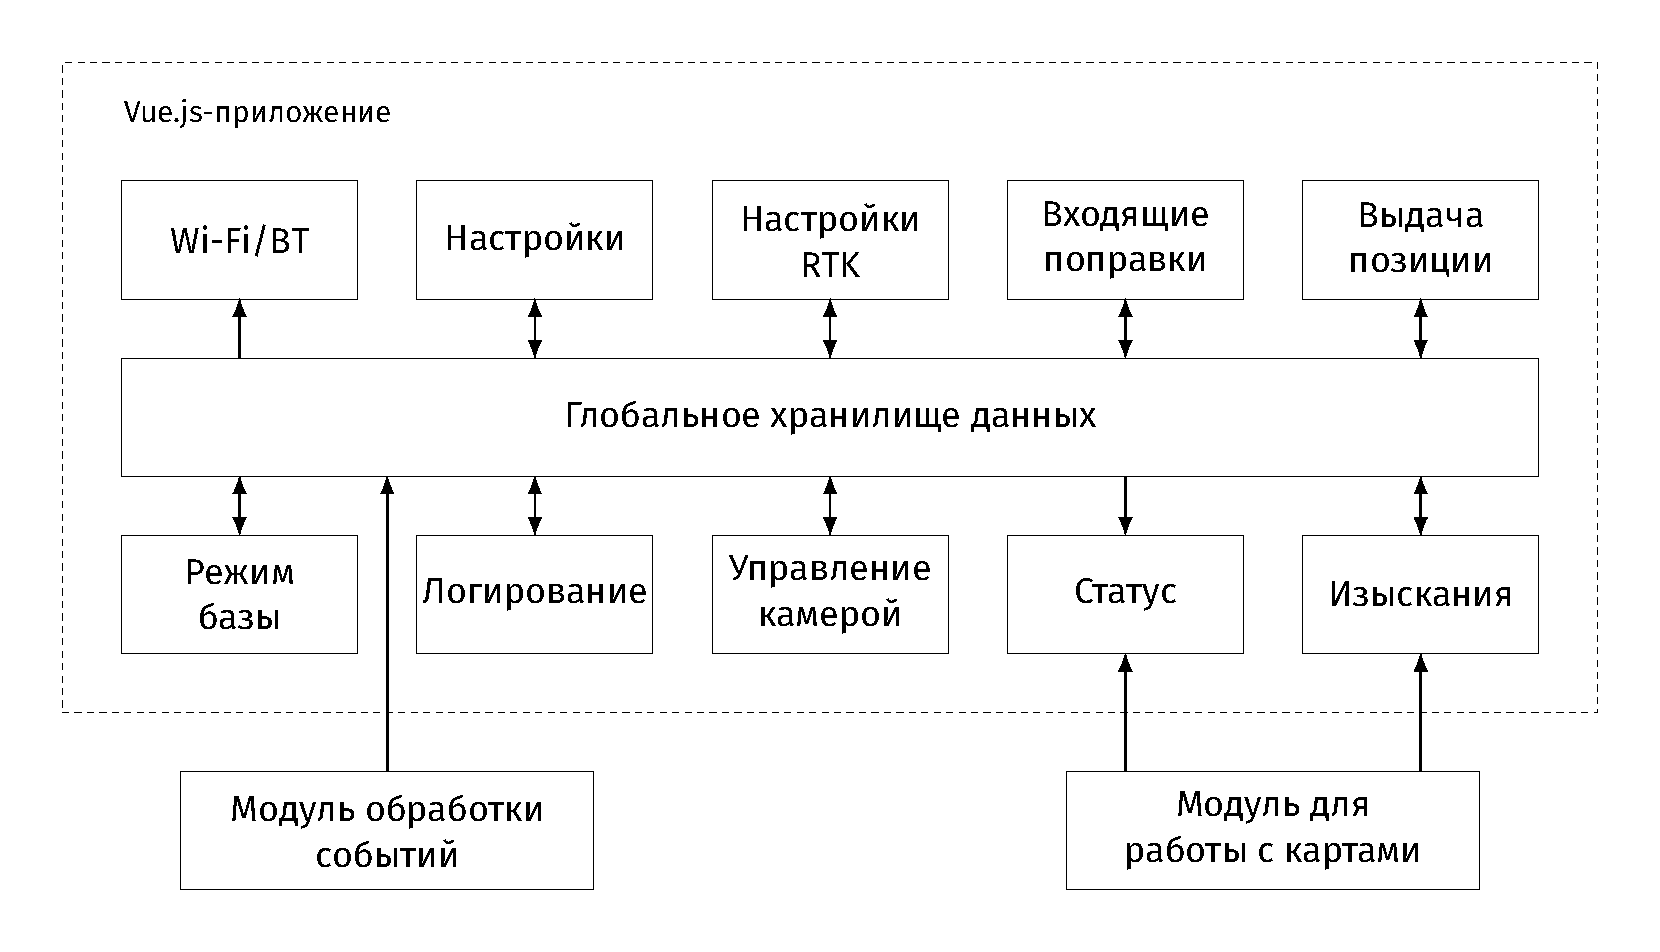
\includegraphics[width=\textwidth]{../../../img/tikz/fe-architecture/pic}
  \caption{Архитектура клиентской части приложения}\label{fig:fe-architecture}
\end{figure}

\mysection{РЕЗУЛЬТАТЫ РАБОТЫ}

\begin{dashitemize}
  \item Проведён обзор платформы для разработки приложения. По результатам обзора используемых устройств были выявлены основные технические особенности, которые необходимо было учесть при разработке клиентского приложения.
  \item На основании ключевых требований к~итоговому приложению и~с~учётом особенностей программного обеспечения используемых устройств, была создана архитектура проекта, а~также были выбраны средства для его реализации.
  \item Была произведена детализация архитектуры клиентской части приложения, в~результате чего были выделены её ключевые модули.
\end{dashitemize}

\end{document}
